% ----------------------------------------------------------
% Introdução (exemplo de capítulo sem numeração, mas presente no Sumário)
% ----------------------------------------------------------
\chapter*{Introdução}
\addcontentsline{toc}{chapter}{Introdução}

Esse relatório tem como objetivo, a partir de ferramentas de simulação de circuitos, mostrar o comportamento de dois circuitos. Além disso, é feito um projeto de uma placa de circuito impressa (PCI) e o cálculo de dimensionamento térmico de um dissipador para o CI LM7805. 

Na simulação dos circuitos, observamaos um filtro passa baixa, que para freqûencias baixas o ganho é próximo de um, e que depois da frequência de corte, seus ganhos tendem a zero. Veremos também um circuito com dois diodos em paralelo. Para a análise destes circuitos, utilizamos o Micro-cap e o PSIM, ambos softwares de simulação de circuitos e vistos anteriormente em outra disciplina.

Para a criação da PCI foi utilizado o software KiCad, as dimensões do indutor utilizado e o tipo de capacitor, podendo ele ser eletrolítico ou cerâmico, foram determinados por dois números, M e N, dados a cada integrante do grupo. Através da média do primeiro número, M, tinha-se a largura do indutor, e a partir do outro, a profundidade. A soma dos dois valores, M+N, determinava o tipo de capacitor, sendo usado um capacitor eletrolítico se a soma der par e um capacitor cerâmico se ímpar.

Finalmente, temos o cálculo de um possível dissipador térmico pra o CI LM7805, para isso utilizamos o \textit{datasheet} do mesmo e cálculos mostrados em aula. 

% ---
\chapter{Ferramentas de Simulação}\label{cap_simul}
% ---
    Para a tarefa 2 proposta da aula 2, temos que primeiramente analisar analiticamente o circuito da figura a). A partir dele, calculamos o $\tau$, $\tau = R*C $, logo $\tau = 1k5 * 100n = 150us$. Para o cálculo da frquência de corte, usamos o valor de $\tau$ anteriormente obtido na fórmula $f = 1/(2\pi\tau)$ e assim a frequência de corte é $f = 1061.033 Hz$. O ganho K, em regime permanente, é dado por $K = Vo/Vi$ onde $Vi$ é a fonte e $Vo$ é a ddp medida no capacitor. Temos, então $K = 1/(1 + 1.5*10^{-4}s)$.
    
    Simulando o circuito a), para achar a frequência de corte:
\begin{figure}[!htb]
    \begin{minipage}{0.5\textwidth}
    \centering
    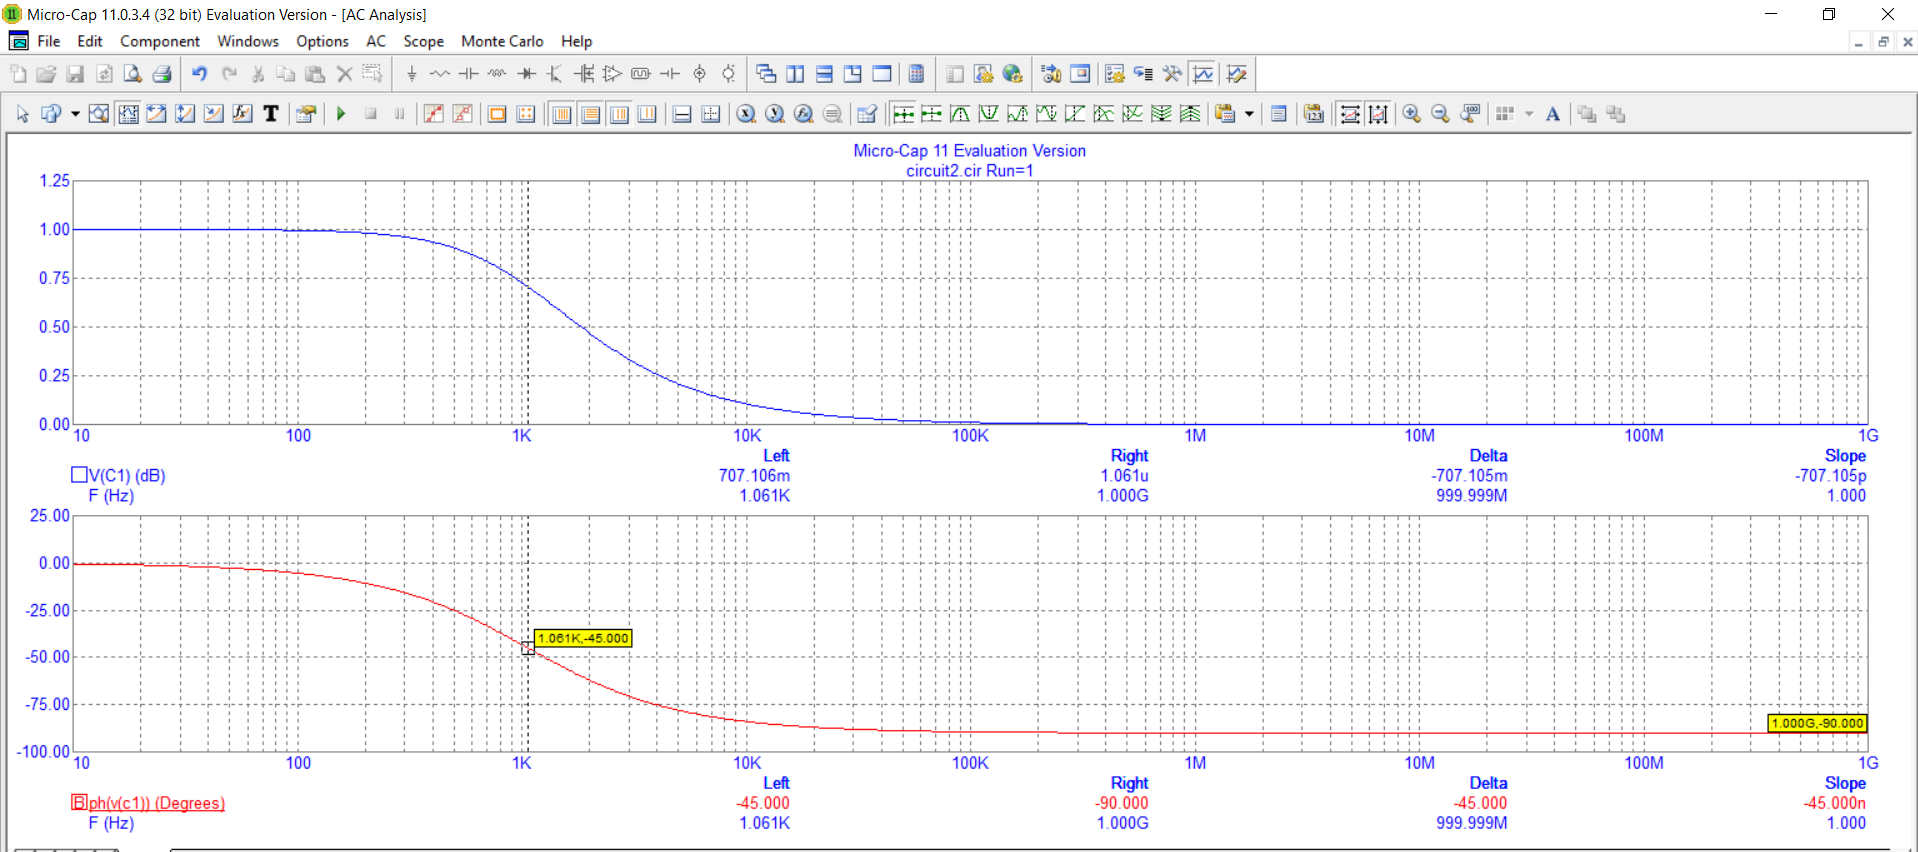
\includegraphics[width = 0.9\textwidth]{Relatorio1_microcap_Bode.png}
    \caption{Simulação no Micro-cap\cite{microcap}}
    \end{minipage}\hfill
    \begin{minipage}{0.5\textwidth}
    \centering
    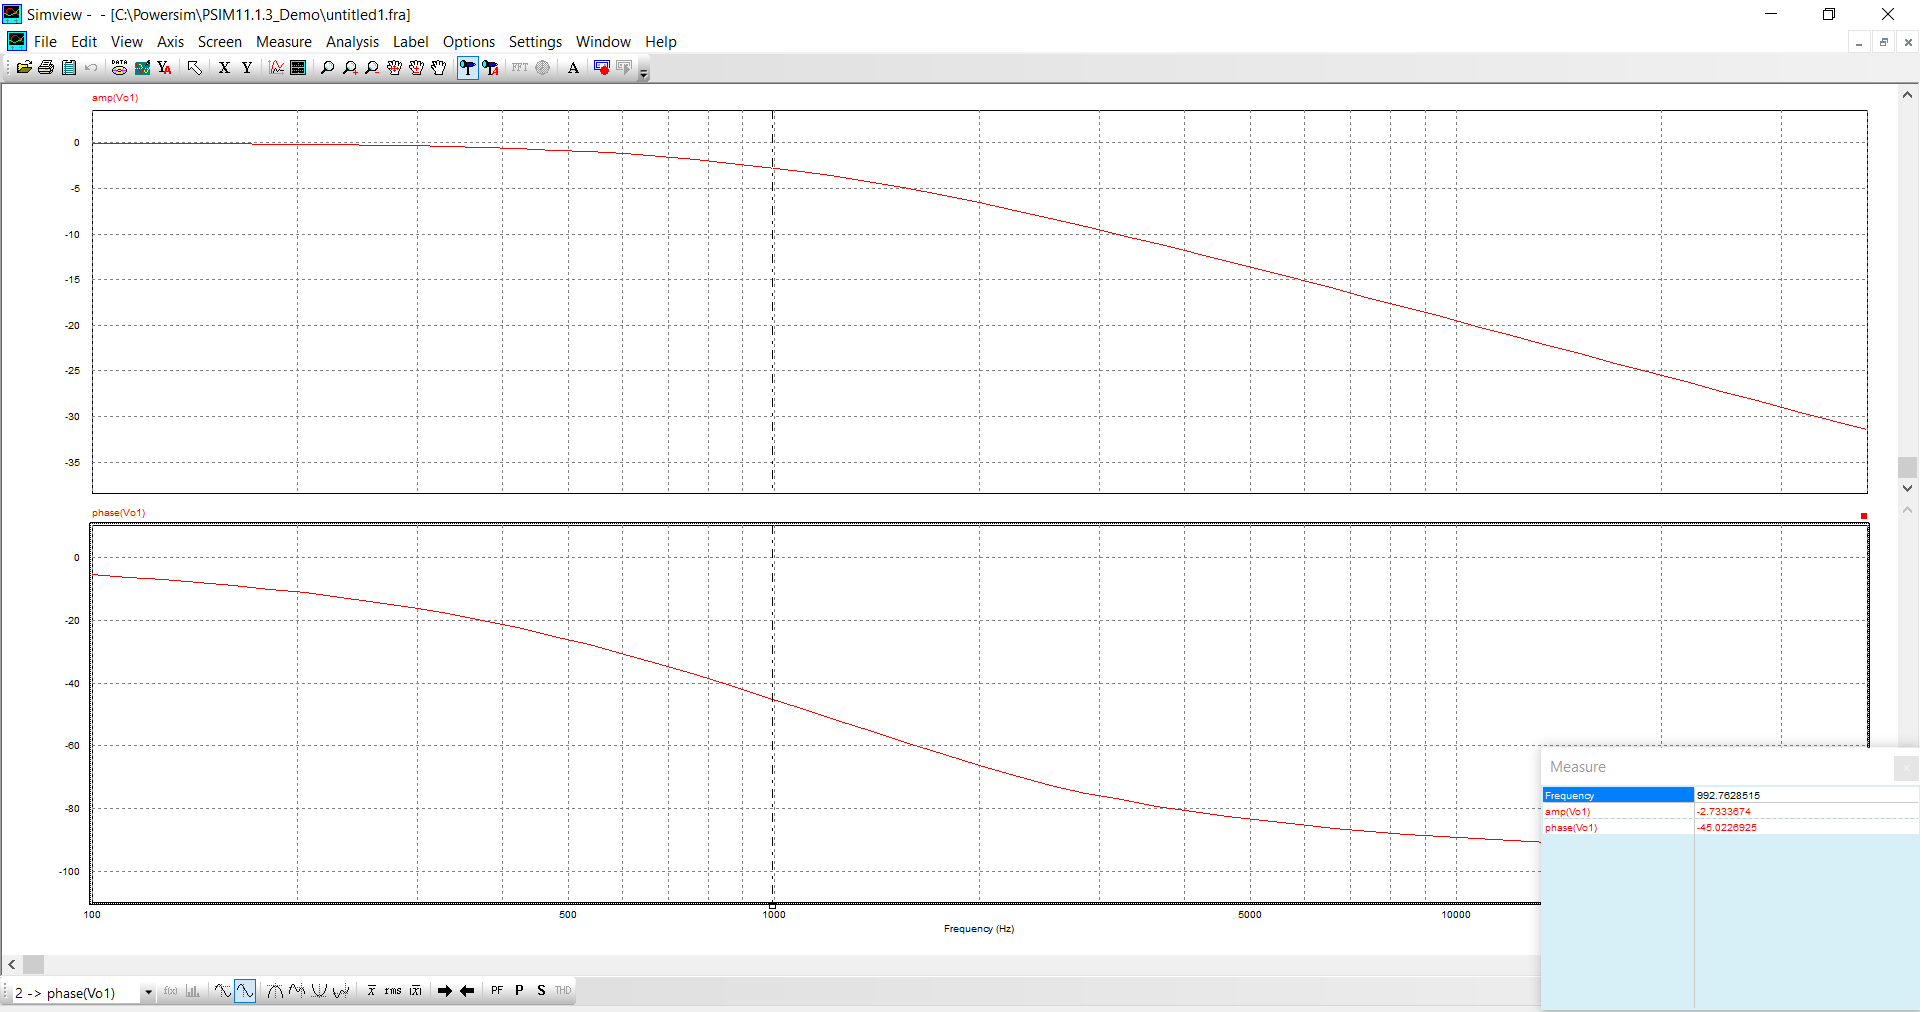
\includegraphics[width = 0.9\textwidth]{Relatorio1_PSIM_Bode.png}
    \caption{Simulação no PSIM\cite{psim}}
    \end{minipage}\hfill
\end{figure}

    Para o resultado do PSIM, mudamos a formade onda para uma senoidal, apenas para o cálcuo da frquência. Com isso, a partir da fase da onda, aos -45graus achamos a frequência de corte em cada simulador. No Micro-cap ficando com 1061Hz e no Psim 992Hz. 
    
    Para encontrar $\tau$, temos:
    
    \begin{figure}[!htb]
    \begin{minipage}{0.5\textwidth}
    \centering
    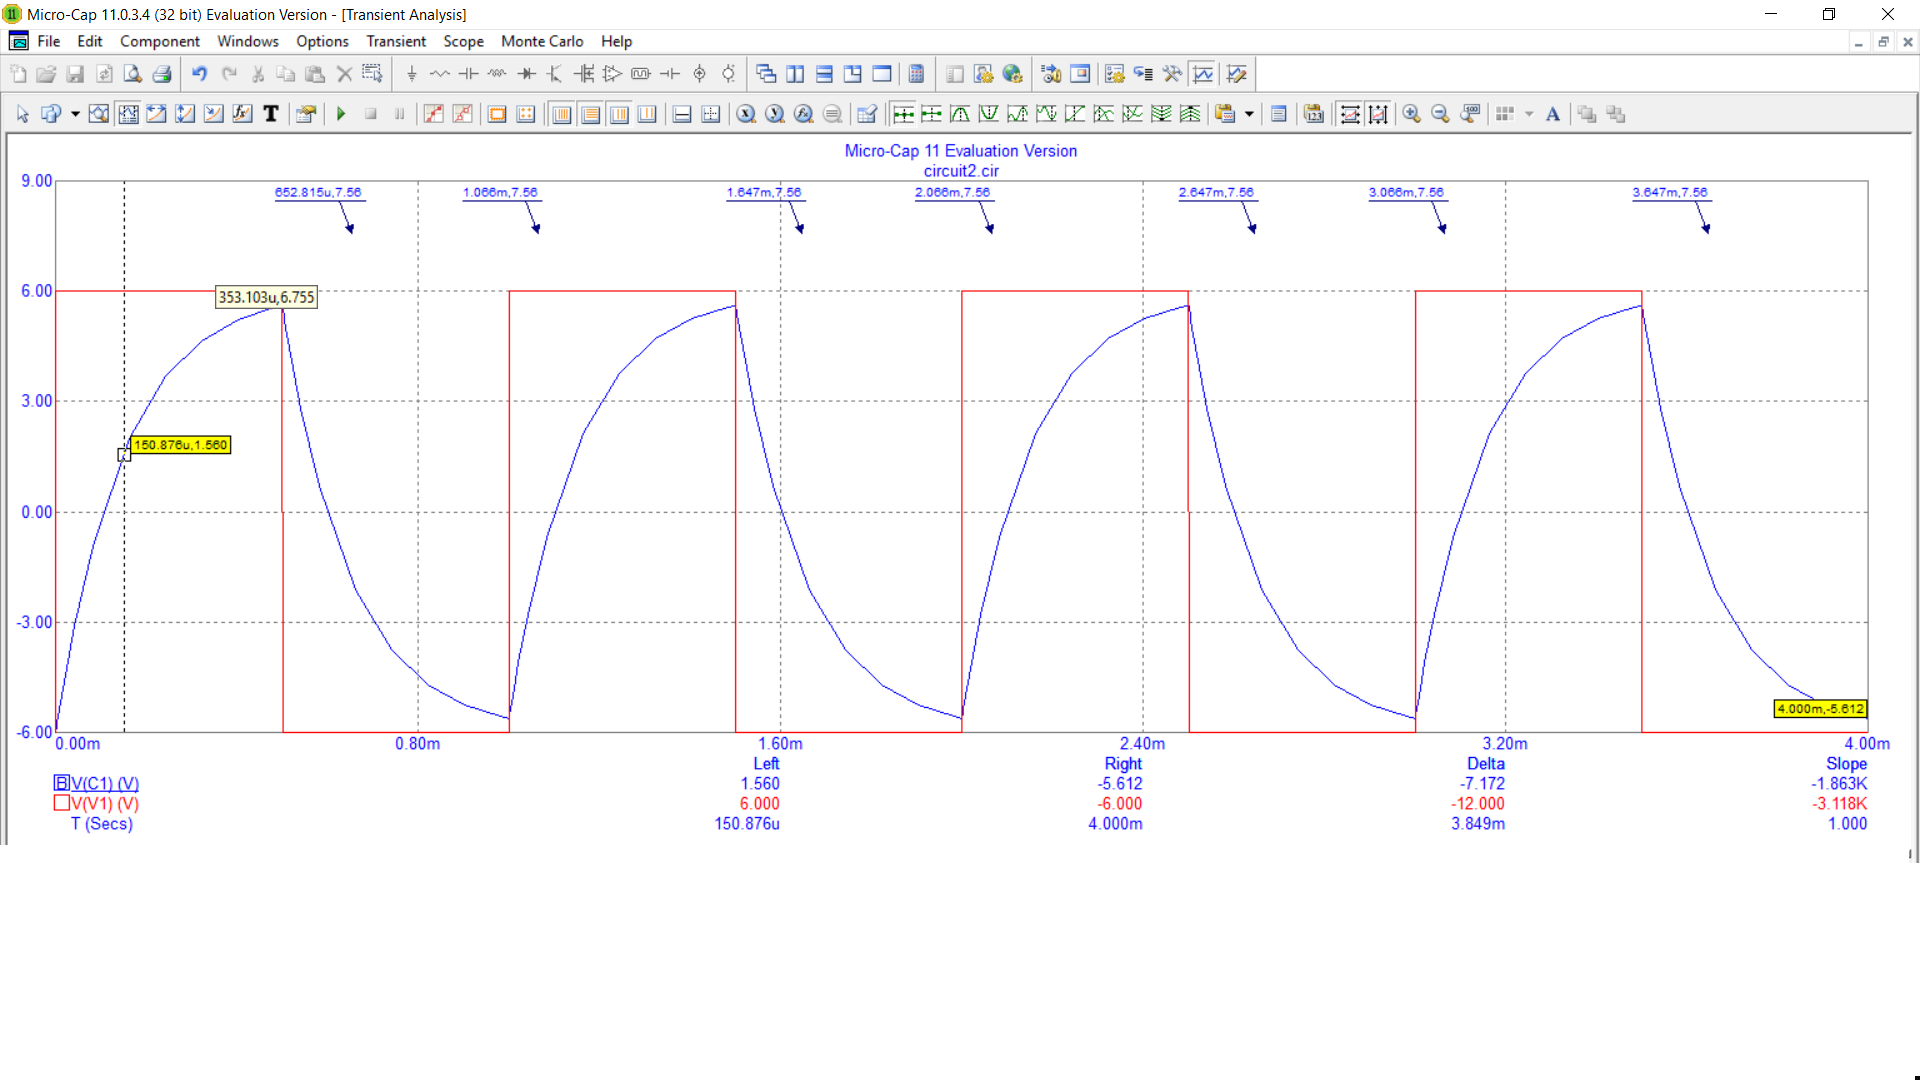
\includegraphics[width = 0.9\textwidth]{Relatorio1_microcap_Tau.png}
    \caption{Simulação no Micro-cap\cite{microcap}}
    \end{minipage}\hfill
    \begin{minipage}{0.5\textwidth}
    \centering
    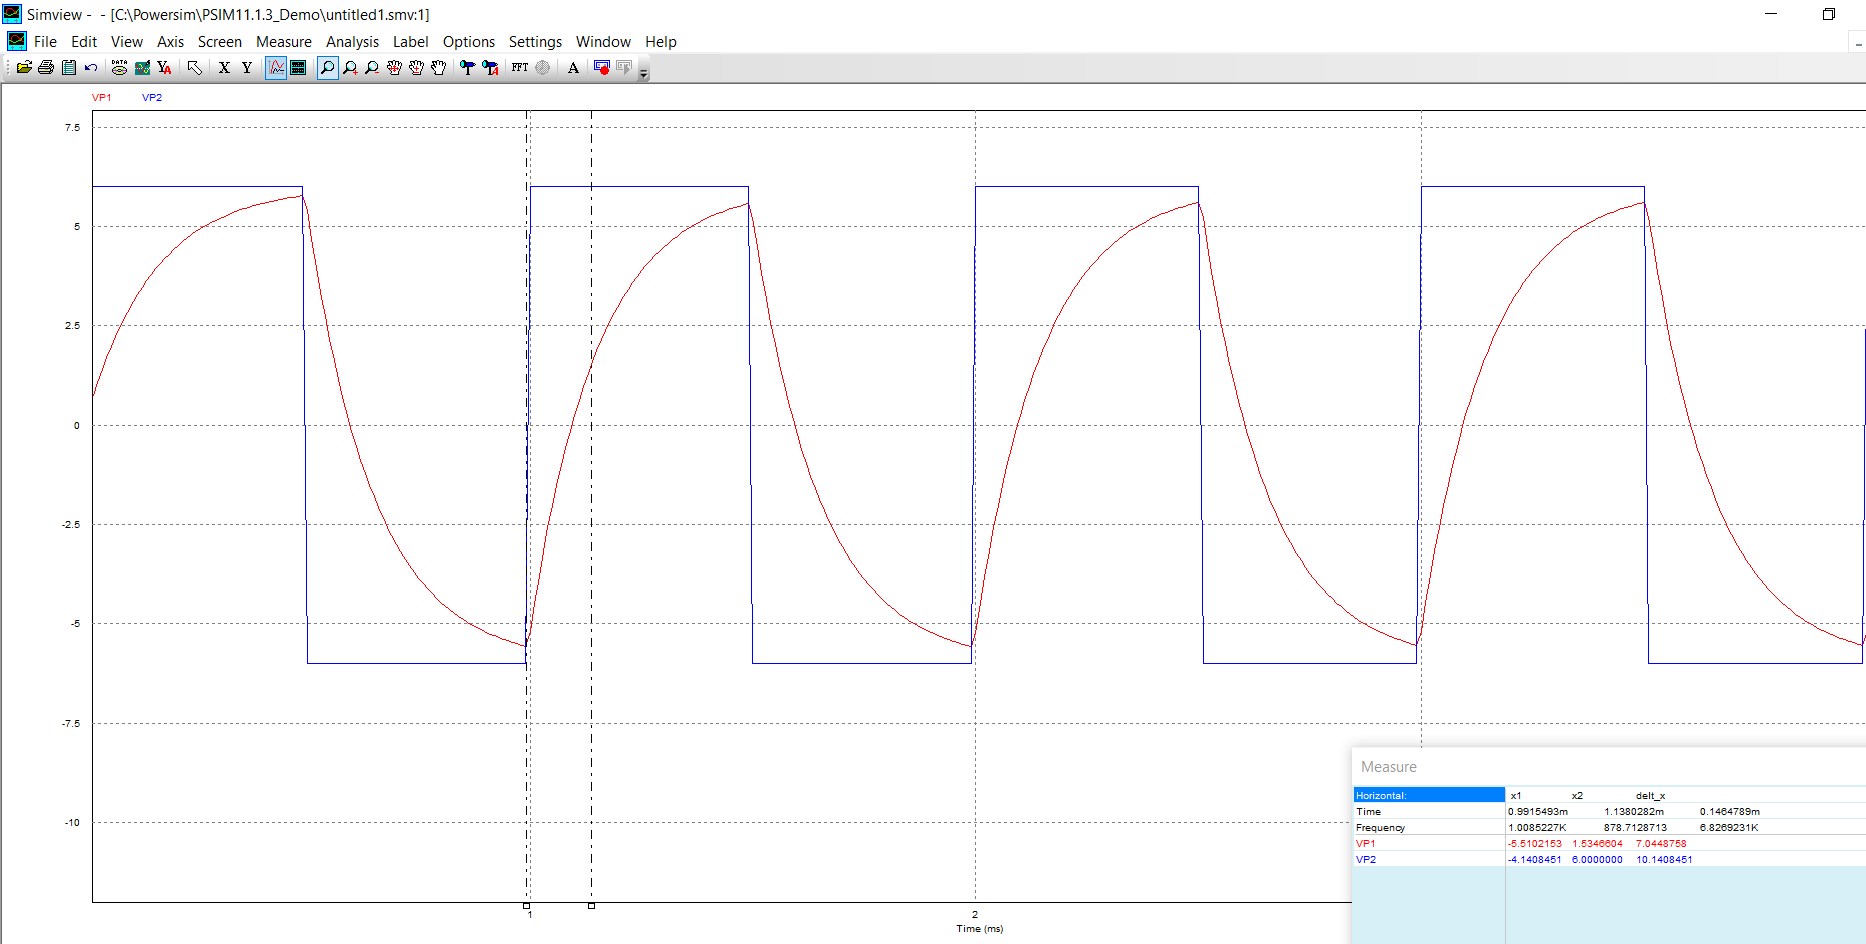
\includegraphics[width = 0.9\textwidth]{Relatorio1_PSIM_Tau.png}
    \caption{Simulação no PSIM\cite{psim}}
    \end{minipage}\hfill
\end{figure}

Para o capacitor carregar 63\% do valor, no micro-cap temos um tempo de 150.876us e no PSIM de aproximadamente 146us. Ambos os simuladores chegaram em resultados parecidos com o esperado, entretanto, pelo fato do Micro-cap ser mais robusto, e não lidar apenas com circuitos ideais, chegou a um resultado mais parecido ao que era esperado.
    
\clearpage
    Para o circuito b), na parte teórica temos o seguinte comportamento:
    
 \begin{figure}[!htb]
    \centering
    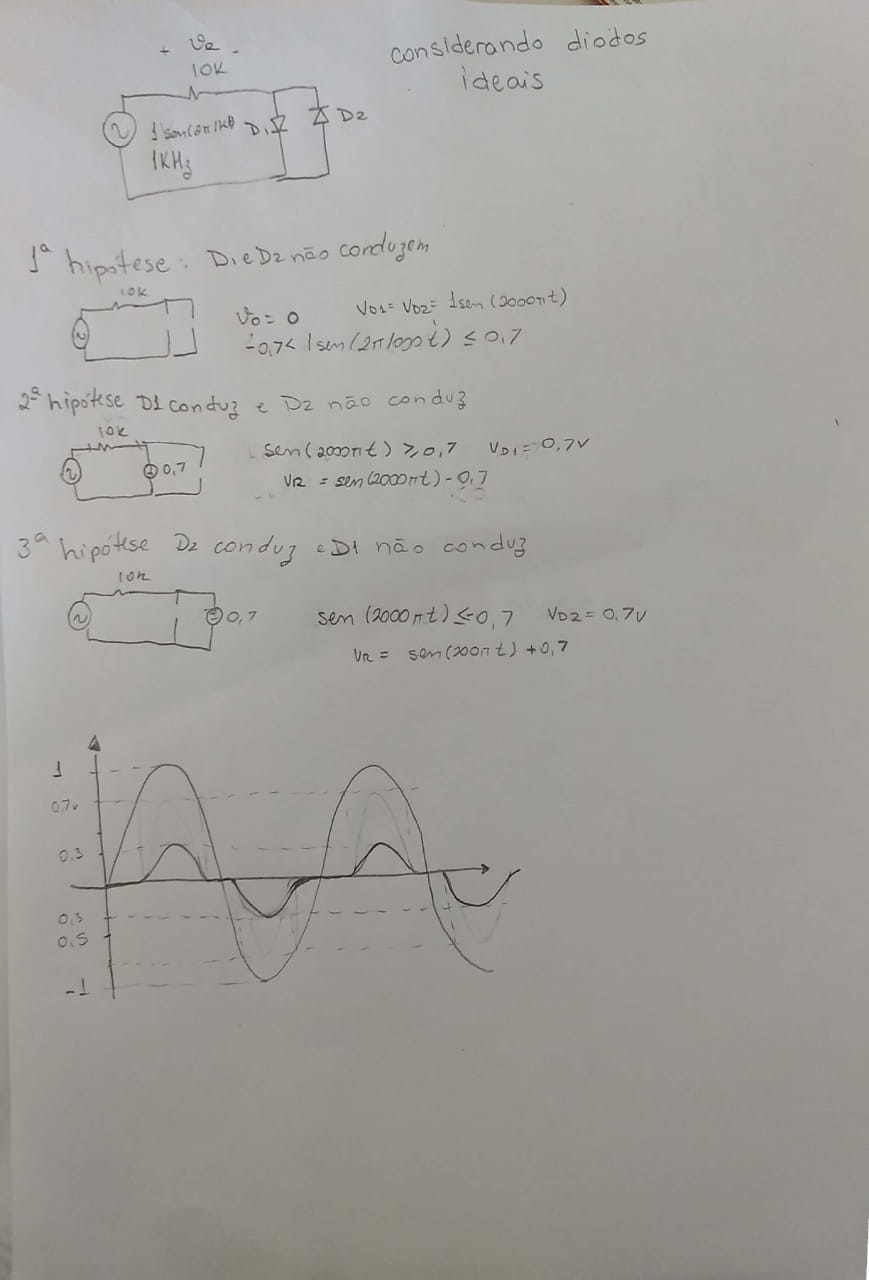
\includegraphics[width=8cm,height=6cm]{Relatorio1_teo_diodo.png}
    \caption{Análise teórica}
\end{figure}
    
    Onde podemos ver que a ddp medida no resistor está em zero até a fonte chegar em 0.7V podendo ser negativo ou positivo e depois disso ela fica a 0.7V a menos que a fonte senoidal. Esse comportamento acontece devido aos diodos em paralelo. Nas simulações, temos:
    
\begin{figure}[!htb]
    \begin{minipage}{0.5\textwidth}
    \centering
    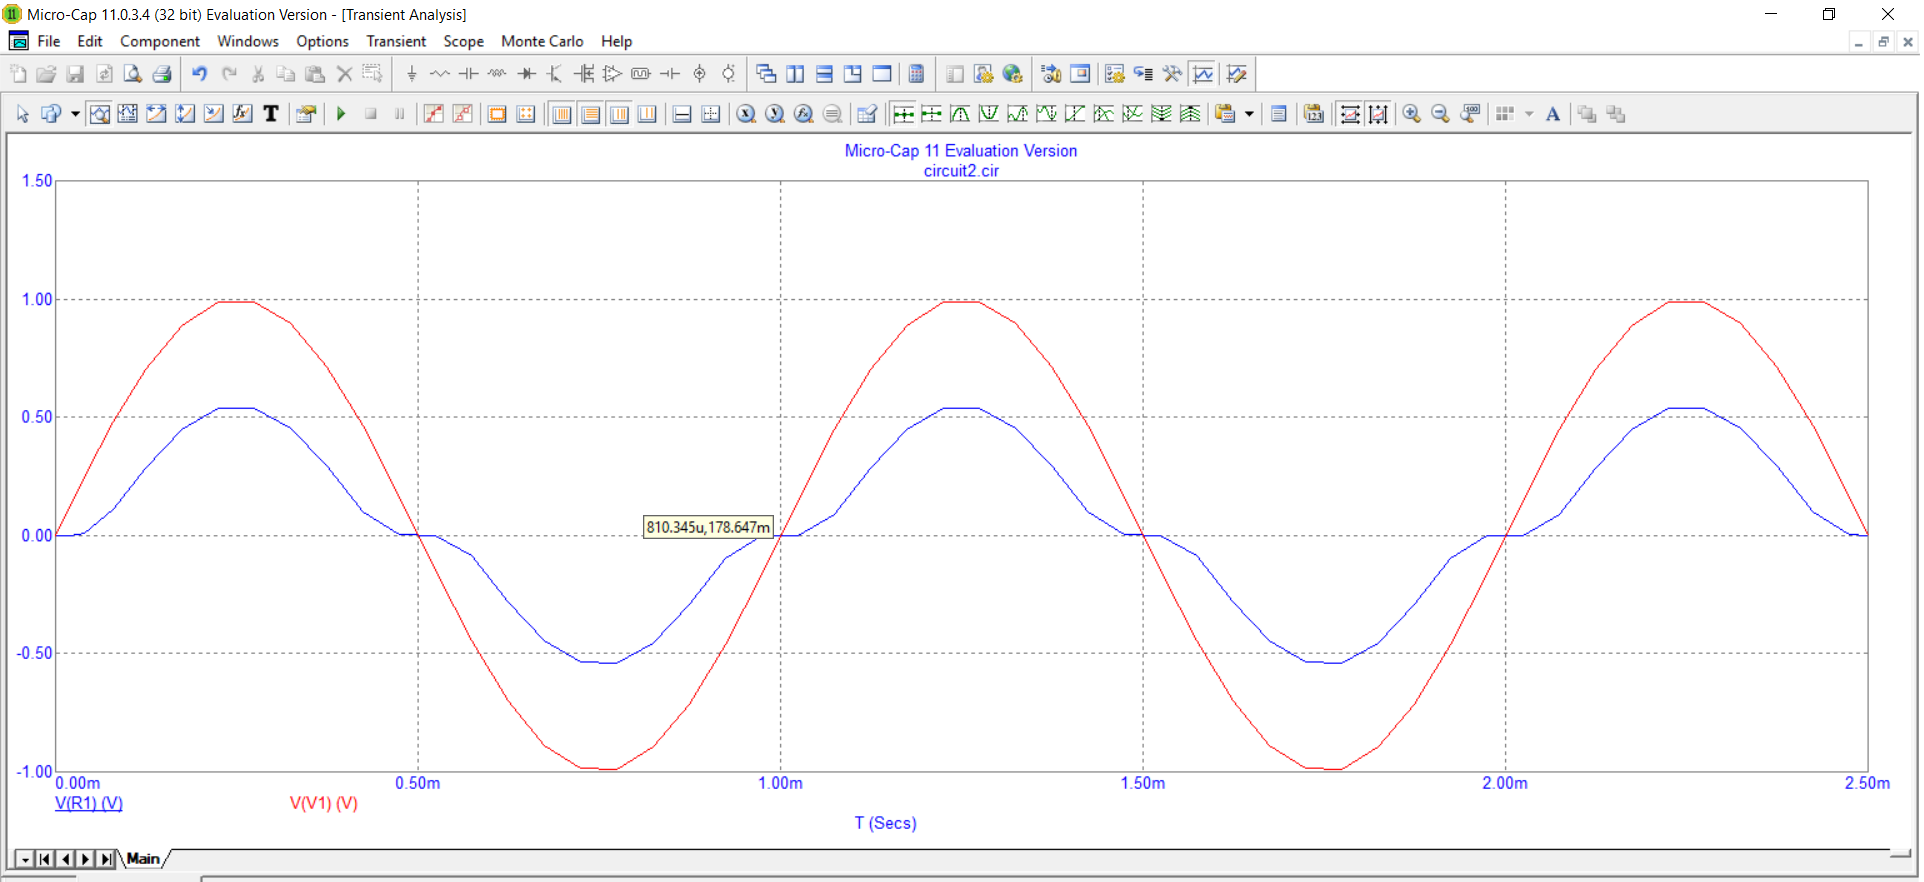
\includegraphics[width = 0.9\textwidth]{Relatorio1_microcap_Diodo.png}
    \caption{Simulação no Micro-cap\cite{microcap}}
    \end{minipage}\hfill
    \begin{minipage}{0.5\textwidth}
    \centering
    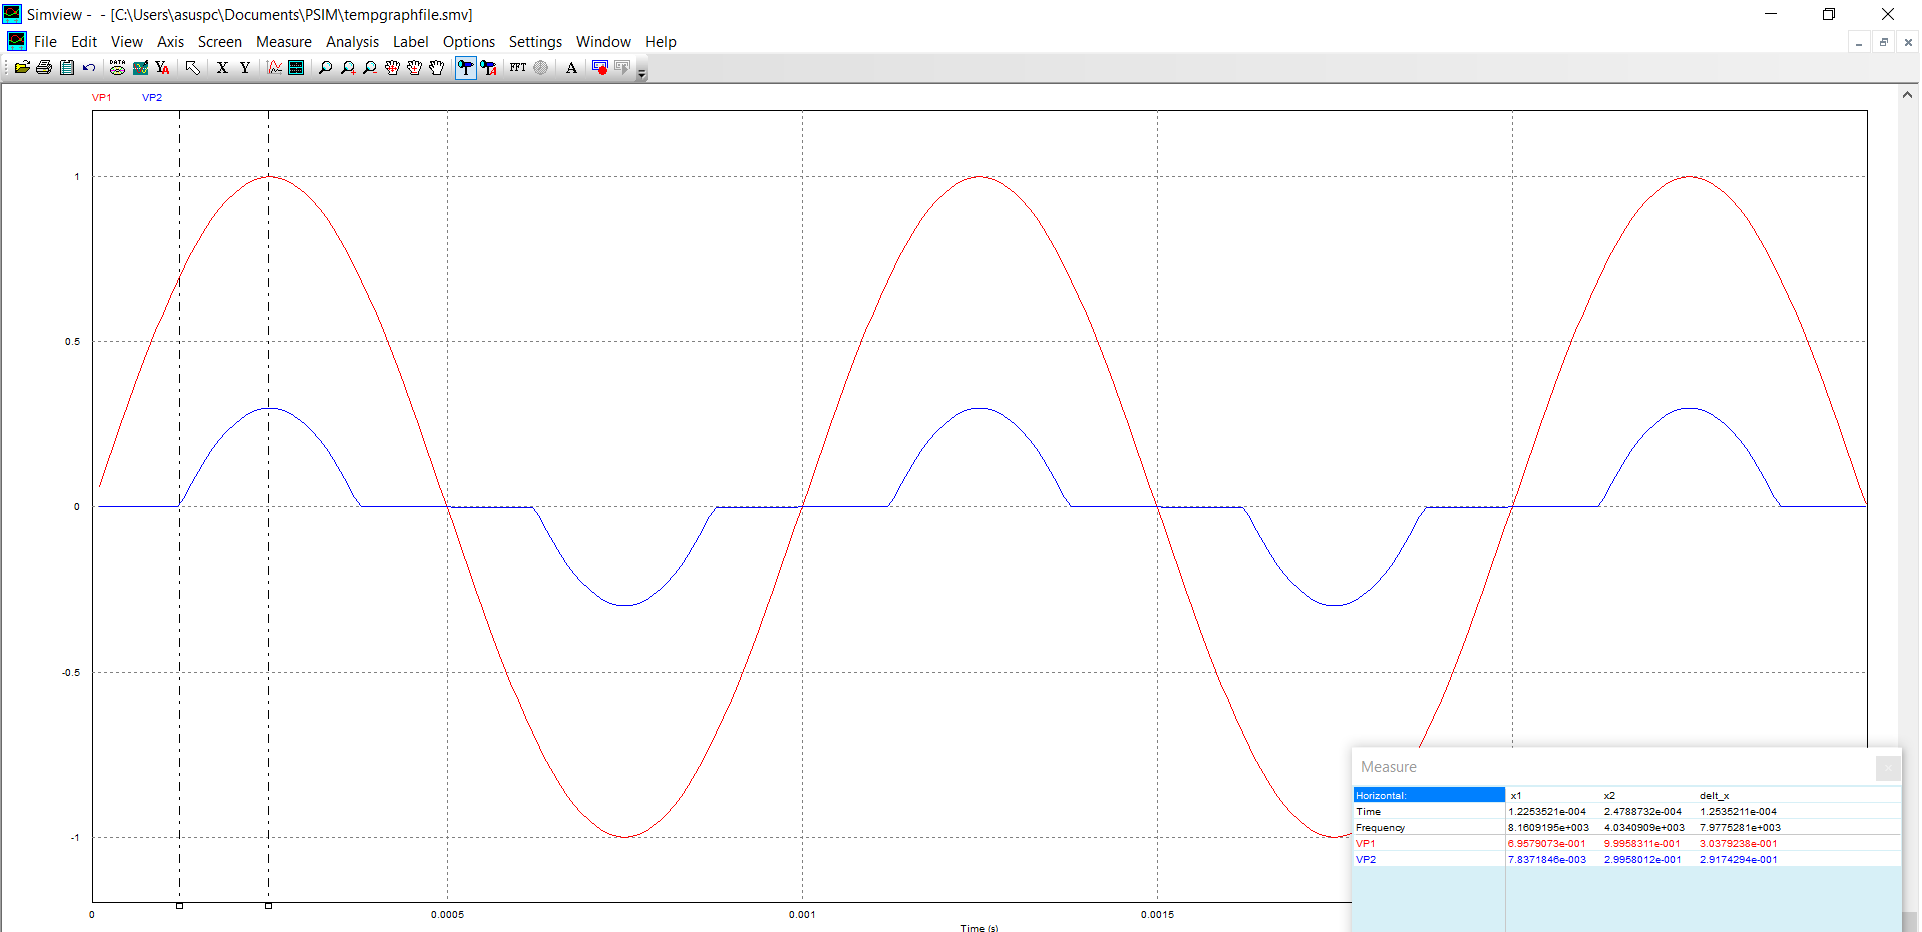
\includegraphics[width = 0.9\textwidth]{Relatorio1_PSIM_Diodo.png}
    \caption{Simulação no PSIM\cite{psim}}
    \end{minipage}\hfill
\end{figure}

  Podemos notar que no PSIM, o resultado ficou muito mais parecido do teórico do que o do Micro-cap. Esse fato ocorre devido ao tipo de diodo utilizado, e o modelo usado pra calcular a forma de onda do mesmo. Na teoria foi utilizado um diodo com 0.7 de \textit{forward voltage} e no PSIM também. Assumimos um comportamento ideal do diodo, logo a resistência interna é zero. Entretanto, no modelo usado no PSIM a resistência interna é de 100m$\Omega$, e o modelo do Micro-cap é o modelo 1N4148.
  
%-----------------------------------------------
%   Projeto de uma Placa de Circuito Impresso 
%
%---------------------------------
\chapter{Projeto de uma Placa de Circuito Impresso }\label{cap_pcb}

Para o projeto da PCI, foi utilizado o software KiCAd\cite{kicad}. Nos era proposto a criação de um circuito RLC, onde o capacitor e o indutor era diferente para cada grupo. Para essa etapa, cada integrante do grupo recebeu dois valores $M$ e $N$, dados pelo professor,fazendo a média dos valores e arredondando para cima, temos novos $M$ e $N$. Esses novos valores que foram utilizados para o dimensionamento do indutor e o tipo de capacitor. No nosso caso, o indutor deveria ter uma altura de 20mm, largura de 50mm e profundidade e 20mm, e nosso capacitor é cerâmico.

\begin{figure}[!htb]
    \begin{minipage}{0.5\textwidth}
    \centering
    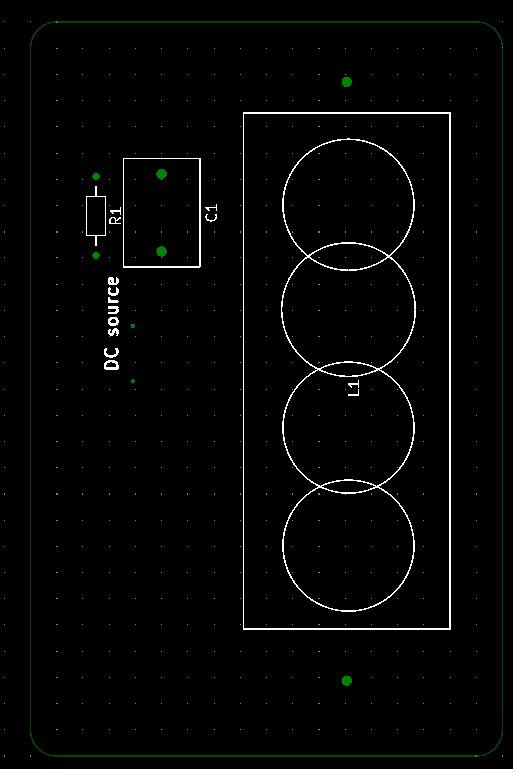
\includegraphics[height = 6cm,width = 0.75\textwidth]{PCB_1.png}
    \caption{Top layer}
    \end{minipage}\hfill
    \begin{minipage}{0.5\textwidth}
    \centering
    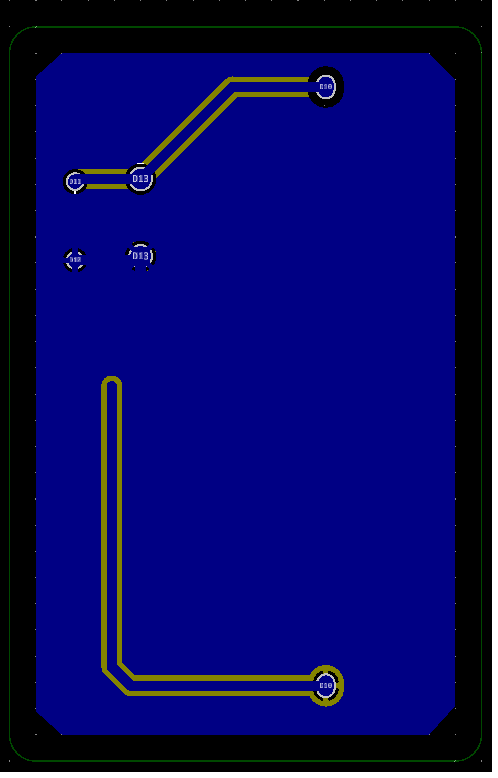
\includegraphics[height = 6cm,width = 0.75\textwidth]{PCB_2.png}
    \caption{Bottom layer}
    \end{minipage}\hfill
\end{figure}

\begin{figure}[!htb]
    \begin{minipage}{0.5\textwidth}
    \centering
    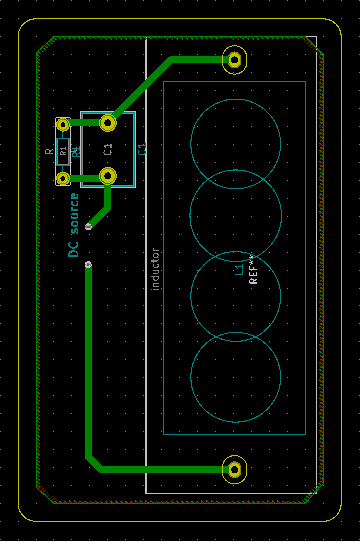
\includegraphics[height = 6cm,width = 0.75\textwidth]{PCB_3.png}
    \caption{Layout}
    \end{minipage}\hfill
    \begin{minipage}{0.5\textwidth}
    \centering
    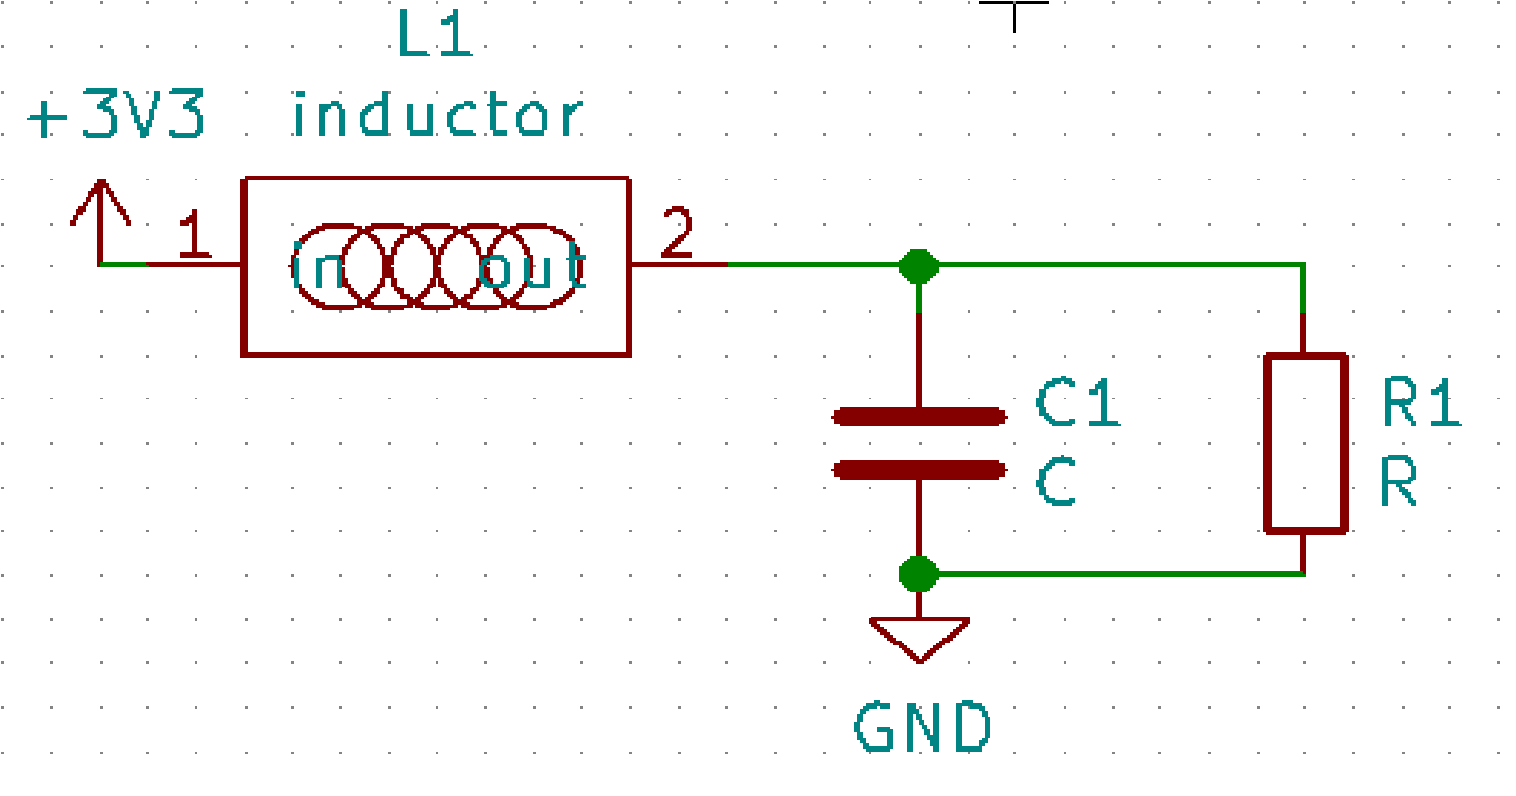
\includegraphics[height = 6cm,width = 0.75\textwidth]{PCB_4.png}
    \caption{Esquemático}
    \end{minipage}\hfill
\end{figure}

\clearpage
Na bottom layer, vemos que não temos uma rota para o ground, isso ocorre porque ela é uma zona preenchida \textit{gnd} assim, só é necessário o ponto de soldagem no capacitor e no resistor para eles estarem conectados ao ground.

%-
%	 Dimensionamento Térmico de um Dissipador 
%
%
\chapter{Dimensionamento Térmico de um Dissipador}

